%%%%%%%%%%%%%%%%%%%%%%%%%%%%%%%%%%%%%%%%%
% Short Sectioned Assignment
% LaTeX Template
% Version 1.0 (5/5/12)
%
% This template has been downloaded from:
% http://www.LaTeXTemplates.com
%
% Original author:
% Frits Wenneker (http://www.howtotex.com)
%
% License:
% CC BY-NC-SA 3.0 (http://creativecommons.org/licenses/by-nc-sa/3.0/)
%
%%%%%%%%%%%%%%%%%%%%%%%%%%%%%%%%%%%%%%%%%

%----------------------------------------------------------------------------------------
%	PACKAGES AND OTHER DOCUMENT CONFIGURATIONS
%----------------------------------------------------------------------------------------

\documentclass[paper=a4, fontsize=11pt]{scrartcl} % A4 paper and 11pt font size

\usepackage[T1]{fontenc} % Use 8-bit encoding that has 256 glyphs
\usepackage{fourier} % Use the Adobe Utopia font for the document - comment this line to return to the LaTeX default
\usepackage[english]{babel} % English language/hyphenation
\usepackage{amsmath,amsfonts,amsthm} % Math packages

\usepackage{graphicx}

\usepackage{sectsty} % Allows customizing section commands
\allsectionsfont{\centering \normalfont\scshape} % Make all sections centered, the default font and small caps

\usepackage{subcaption}
\usepackage{pdfpages}
\usepackage{float}
\usepackage{url}

\usepackage{fancyhdr} % Custom headers and footers
\pagestyle{fancyplain} % Makes all pages in the document conform to the custom headers and footers
\fancyhead{} % No page header - if you want one, create it in the same way as the footers below
\fancyfoot[L]{} % Empty left footer
\fancyfoot[C]{} % Empty center footer
\fancyfoot[R]{\thepage} % Page numbering for right footer
\renewcommand{\headrulewidth}{0pt} % Remove header underlines
\renewcommand{\footrulewidth}{0pt} % Remove footer underlines
\setlength{\headheight}{13.6pt} % Customize the height of the header

\numberwithin{equation}{section} % Number equations within sections (i.e. 1.1, 1.2, 2.1, 2.2 instead of 1, 2, 3, 4)
\numberwithin{figure}{section} % Number figures within sections (i.e. 1.1, 1.2, 2.1, 2.2 instead of 1, 2, 3, 4)
\numberwithin{table}{section} % Number tables within sections (i.e. 1.1, 1.2, 2.1, 2.2 instead of 1, 2, 3, 4)

\setlength\parindent{0pt} % Removes all indentation from paragraphs - comment this line for an assignment with lots of text

%----------------------------------------------------------------------------------------
%	TITLE SECTION
%----------------------------------------------------------------------------------------

\newcommand{\horrule}[1]{\rule{\linewidth}{#1}} % Create horizontal rule command with 1 argument of height

\title{	
\normalfont \normalsize 
\textsc{Bonn-Rhein-Sieg University of Applied Sciences} \\ [25pt] % Your university, school and/or department name(s)
\horrule{0.5pt} \\[0.4cm] % Thin top horizontal rule
\huge Scientific Experimentation and Evaluation\\
- Assignment 04 - \\ 
Camera Calibration Setup\\% The assignment title
\horrule{2pt} \\[0.5cm] % Thick bottom horizontal rule
}

\author{Mazin Eltayeb, Bastian Lang} % Your name

\date{\normalsize\today} % Today's date or a custom date

\begin{document}

\maketitle % Print the title

\tableofcontents
\newpage

\section{Abstract}
%Read and understand the papers from Zhang and Heikkil (provided in LEA). Based on your
%understanding of camera calibration, design a calibration setup and detail the actual calibration
%process.
%Test the provided camera on your laptop and ensure you can capture still images.
%Deliverables 3.1
%Write a design report describing the calibration process, including a theoretical part that describes
%the camera and lens errors measured and corrected by the calibration. Your design report should
%cover:
%1. A description of the setup for calibration, including possible pitfalls.
%2. An estimation of the number of images and image positions required.
%3. a description of the parameters (what do they mean?) calculated by the Matlab calibration
%toolbox.
%4. Discuss possible problems or error sources that can disturb the calibration process. Include
%any observation you may have made while testing the proper functioning of the camera with
%your laptop.
This report describes the design of the camera calibration process, including its setup, the calibration parameters and possible problems during the calibration.

\section{Setup}
The camera will be fixed in its position by securing it on a solid surface with some tape.
The chessboard pattern used for the calibration will be fixed on a flat board. 
The board will be held in hands and changed in orientation with respect to the camera for every image.
In the online tutorial (\cite{tutorial}) 20 images were sufficient, we also plan to use about 20-25 images.
The orientations of the images should differ for each image and provide a good range of different orientations.

\section{Camera Parameters}
Matlab computes the following parameters:
\begin{itemize}
	\item \textbf{Focal Length} (2x1 vector)\\
	"The focal length of an optical system is a measure of how strongly the system converges or diverges light." \cite{wiki} (see figure \ref{ref_focal}).
	
	\item \textbf{Principal Point} (2x1 vector)\\
	"The principal points are the points where the principal planes cross the optical axis."\cite{wiki}\\
	"The two \textbf{principal planes} have the property that a ray emerging from the lens appears to have crossed the rear principal plane at the same distance from the axis that that ray appeared to cross the front principal plane, as viewed from the front of the lens. This means that the lens can be treated as if all of the refraction happened at the principal planes."\cite{wiki} (see figure \ref{ref_principal}).
	
	\item \textbf{Skew Coefficient} (scalar)\\
	"The skew coefficient defines the angle between the x and y pixel axes"\cite{calibration}
	
	
	\item \textbf{Distortions} (5x1 vector)\\
	Matlab stores both radial and tangential distortions in the distortions vector.\cite{calibration}\\
	Radial distortions increase or decrease magnification with the distance to the optical axis\cite{wiki}(see figure \ref{ref_radial}).\\
	Tangential distortion occurs when camera lens and sensor are not parallel (see figure \ref{ref_tangential}).
	
	\item \textbf{Rotations} (set of 3x3 rotation matrices)\\
	Rotations from images into reference frame.\cite{calibration}
	
	\item \textbf{Translations} (set of 3x1 vectors)\\
	Coordinate vectors of the origin of the grid pattern in camera reference frame. \cite{calibration}
	
\end{itemize}


\begin{figure}[H]
	\centering
	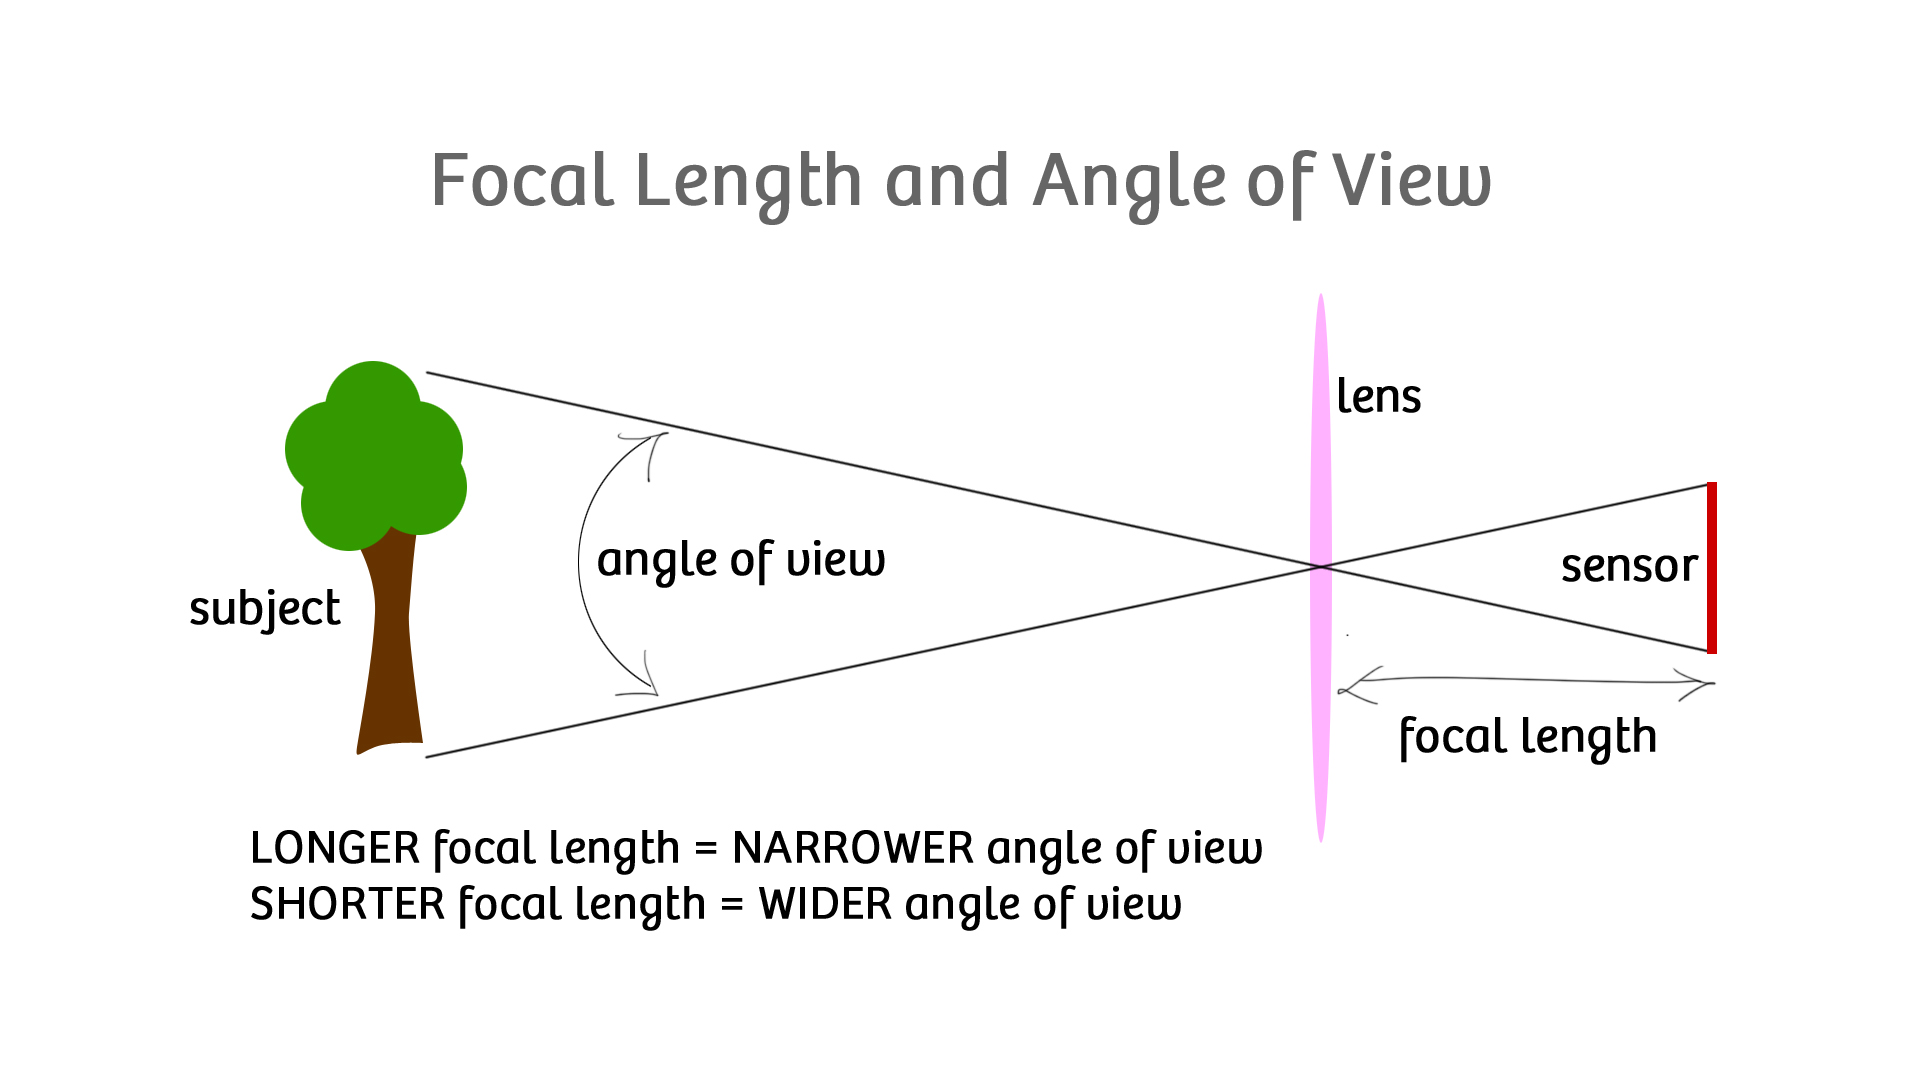
\includegraphics[width = 0.6\linewidth]{focal_length.jpg}
	\caption{Focal Length, \\http://static.snapsnapsnap.photos/wp-content/uploads/2014/11/Focal-Length-and-Angle-of-View.jpg}
	\label{ref_focal}
\end{figure}

\begin{figure}[H]
	\centering
	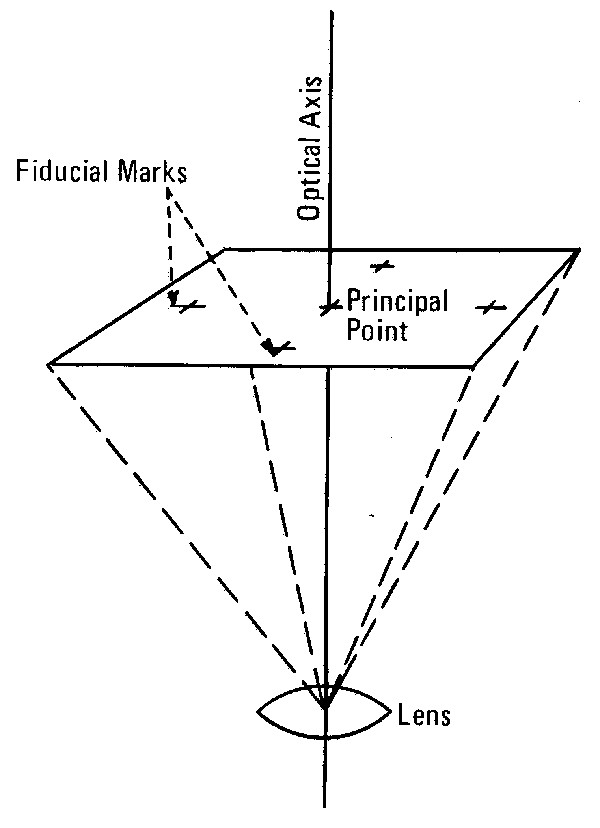
\includegraphics[width = 0.6\linewidth]{principal.jpg}
	\caption{Principal Point, \\http://www.fao.org/docrep/003/t0390e/T0390E48.gif}
	\label{ref_principal}
\end{figure}

\begin{figure}[H]
	\centering
	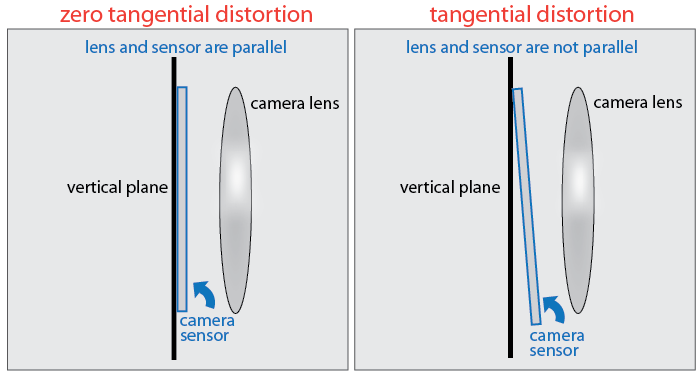
\includegraphics[width = 0.6\linewidth]{tangential.png}
	\caption{Tangential Distortion, \\http://www.mathworks.com/help/vision/ref/cameracalibrator\textunderscore tangentialdistortion.png}
	\label{ref_tangential}
\end{figure}

\begin{figure}[H]
	\centering
	
\includegraphics[width = 0.6\linewidth]{radial.png}
	\caption{Radial Distortion, \\http://www.intechopen.com/source/html/44946/media/image17.png}
	\label{ref_radial}
\end{figure}

\section{Possible Problems}
One problem could be surface of the grid if it is not fixated on the plate properly. 
This could lead to unwanted bending of the grid.
Another problem could occur if the grid is not being held still while taking the pictures.
The images could become blurred and useless.
If the checker board gets partly out of the image these images will become useless as well.
The lighting conditions need to be good to ensure the distinction of the single checker cells.




\bibliographystyle{plain}
\bibliography{bibtex.bib}






\end{document}